\section{粒子群优化算法}

\subsection{标准PSO}

粒子群优化（Particle Swarm Optimization, PSO）
由Kennedy和Eberhart于1995年提出，
是一种基于群体智能的元启发式优化算法。
在标准PSO中，每个粒子维护自身的历史最优解$p_i$
和全局最优解$g$，
通过以下公式更新速度和位置：

\begin{equation}
    v_i^{t+1} = w v_i^t + c_1 r_1 (p_i - x_i^t) + c_2 r_2 (g - x_i^t)
    \label{eq:pso_velocity}
\end{equation}

\begin{equation}
    x_i^{t+1} = x_i^t + v_i^{t+1}
    \label{eq:pso_position}
\end{equation}

其中：
\begin{itemize}
    \item $v_i^t$：粒子$i$在第$t$代的速度向量；
    \item $x_i^t$：粒子$i$在第$t$代的位置向量；
    \item $w$：惯性权重，控制搜索的探索-利用平衡；
    \item $c_1, c_2$：个体学习和群体学习因子（标准值1.5--2.0）；
    \item $r_1, r_2$：$[0,1]$上的随机数，引入随机扰动。
\end{itemize}

\subsection{自适应惯性权重改进}

标准PSO使用固定惯性权重$w$，
难以在探索（大$w$）和利用（小$w$）之间自适应切换。
本课题引入自适应惯性权重策略：

\begin{equation}
    w(t) = w_{\text{max}} - (w_{\text{max}} - w_{\text{min}}) \cdot \frac{t}{T_{\text{max}}}
    \label{eq:adaptive_w}
\end{equation}

其中$w_{\text{max}} = 0.9$，$w_{\text{min}} = 0.4$，
$t$为当前迭代数，$T_{\text{max}}$为最大迭代数。
线性递减策略使PSO在早期维持较强的全局探索能力，
后期集中于局部精细搜索。

\subsection{不确定性感知的风险敏感适应度（创新点①）}

本课题将\textbf{不确定性感知（Uncertainty-Aware）思想引入PSO框架}，
利用DeepEnsemble的不确定性估计能力，
将PSO的标准目标函数扩展为：

\begin{equation}
    \text{Fitness}(x) = \mu(x) - \lambda \cdot \sigma(x) - P_{\text{scenario}}(x)
    \label{eq:risk_sensitive}
\end{equation}

该公式同时解决三个关键问题：

\begin{enumerate}
    \item \textbf{OOD防护}：当PSO粒子进入训练数据稀疏的分布外（OOD）区域时
        （本文以DeepEnsemble的$\sigma(x)$不确定性估计作为OOD的代理指标，
        并非形式化的分布外检测方法——更准确的表述是"低密度/高不确定性区域"），
        DeepEnsemble的$\sigma(x)$显著增大，
        $\lambda\sigma(x)$项产生惩罚，
        使粒子自然返回可靠区域；
    \item \textbf{不平衡缓解}：低稳定性样本在原数据集中的稀疏性
        导致代理模型对低稳定性预测范围的不确定性更高，
        $\sigma(x)$惩罚使PSO避免单纯追求名义高分而忽视模型可信度；
    \item \textbf{幻觉抑制}：代理模型可能在OOD区域输出虚假的高分
        （幻觉），$\sigma(x)$惩罚提供了一种模型自知的可靠性过滤。
\end{enumerate}

风险厌恶系数$\lambda$控制保守程度。
$\lambda = 0$退化为标准最大化$\mu(x)$（无风险防护）；
$\lambda$越大，PSO越倾向于搜索模型置信度高的区域。

需要指出的是，
$\mu(x)-\lambda\sigma(x)$形式的适应度函数在方法论上与贝叶斯优化中的
Lower Confidence Bound（LCB）采集函数$f(x^*)=\mu(x)-\beta\sigma(x)$
和上置信界（UCB）思想共享数学形态。
然而，本方法与LCB/UCB存在本质区别：
\begin{itemize}
    \item \textbf{应用目标不同}：LCB/UCB作用于代理模型的采样策略，
        目的是在探索与利用之间平衡采样效率；
        本方法的$\lambda\sigma(x)$惩罚则是\textbf{直接内嵌于优化目标函数}，
        通过PSO群体的协同搜索实现面向可靠性的约束寻优；
    \item \textbf{信息来源不同}：本方法的$\sigma(x)$来自
        DeepEnsemble的成员间预测分歧（非参数不确定性），
        而非高斯过程的后验方差（模型不确定性）；
    \item \textbf{优化机制不同}：PSO的群体搜索天然具备多样性维护能力，
        与$\sigma(x)$惩罚形成协同——
        粒子在遇到高不确定性区域时会自然折返，
        无需额外的采集函数规划。
\end{itemize}

因此，准确的方法论定位是：
\textbf{本文将不确定性感知思想引入PSO群体智能框架}，
而非提出全新的优化范型。$\sigma(x)$惩罚在PSO语境下的核心价值
在于将代理模型的可靠性自知内化为优化过程的约束条件，
这对于数据驱动优化中的OOD可靠性保障具有重要的工程实践意义。

\subsection{PSO配置总结}

\begin{table}[H]
\centering
\caption{PSO超参数配置}
\begin{tabular}{lrl}
\toprule
参数 & 值 & 说明 \\
\midrule
粒子数 $N$ & 50 & 权衡搜索广度与计算效率 \\
最大迭代数 $T_{\text{max}}$ & 80 & 满足需求收敛目标 \\
惯性权重 $w$ & 0.9 $\to$ 0.4 (线性递减) & 自适应平衡探索-利用 \\
学习因子 $c_1$ & 2.0 & 个体经验权重 \\
学习因子 $c_2$ & 1.5 & 群体经验权重 \\
风险系数 $\lambda$ & 1.0 & 中等风险厌恶 \\
收敛判定 & stall $\geq$ 12代 & gbest连续12代无改善即终止 \\
\bottomrule
\end{tabular}
\end{table}

\subsection{PSO收敛分析}

\begin{figure}[H]
\centering
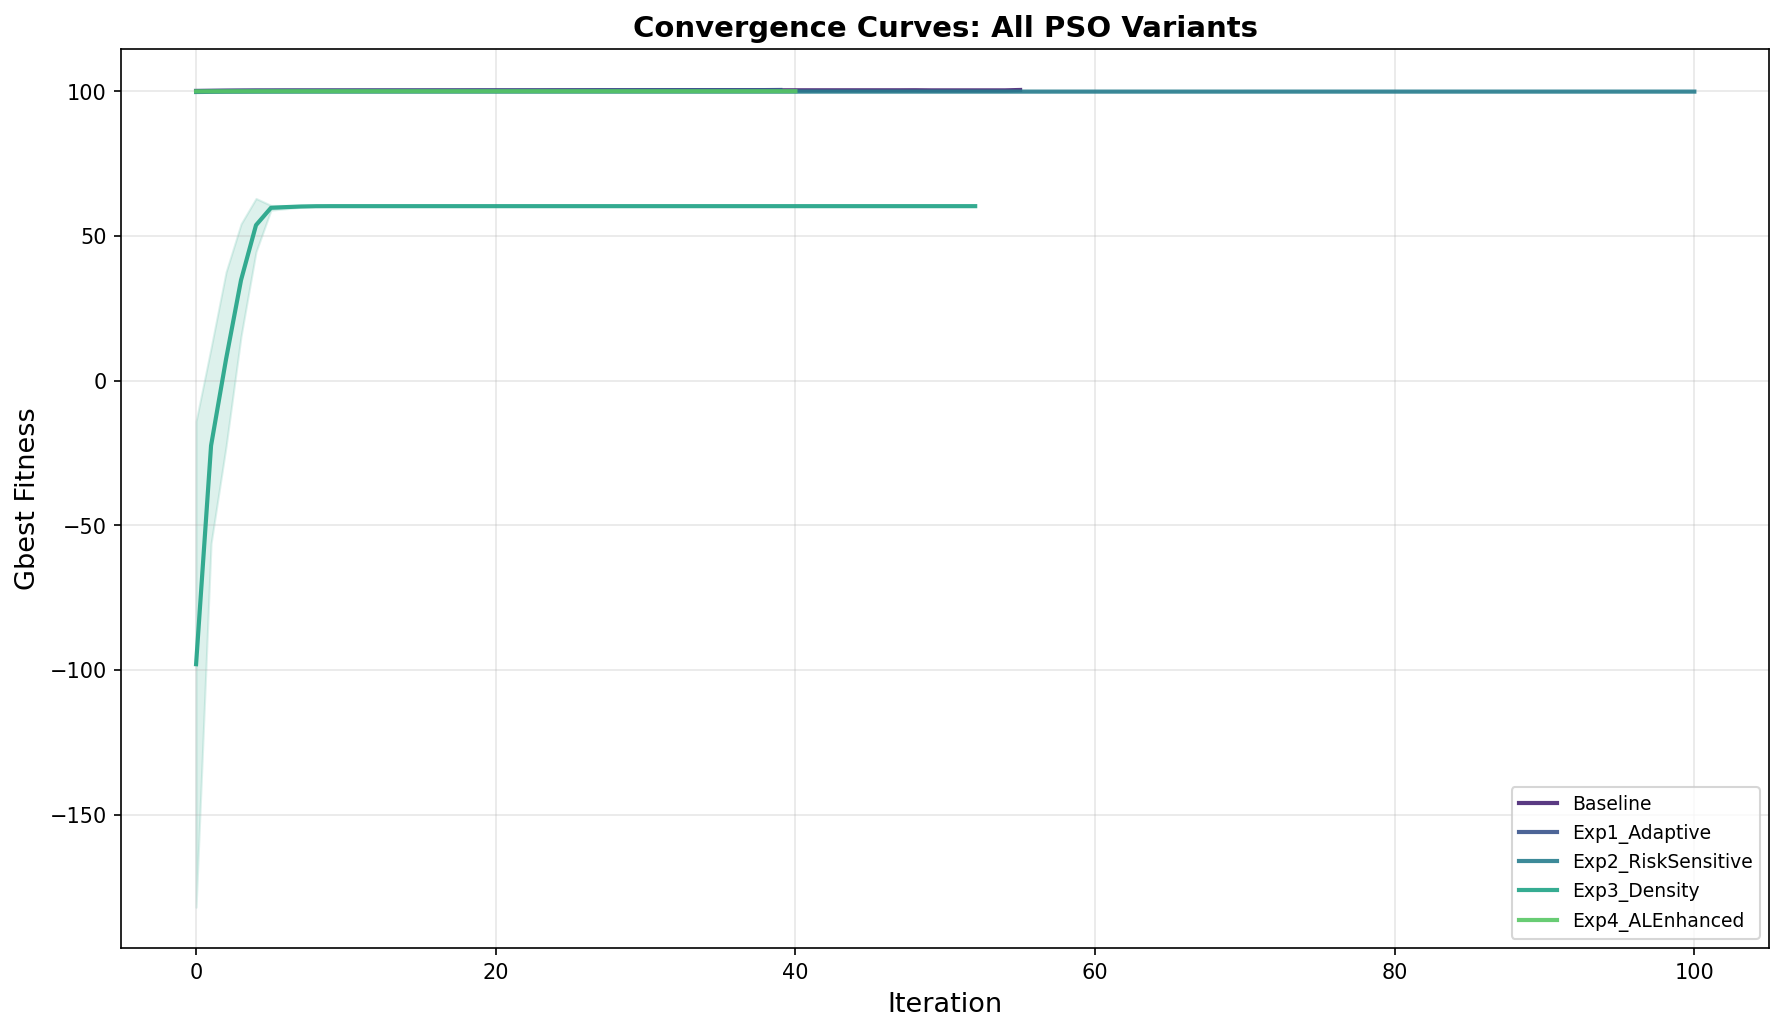
\includegraphics[width=0.78\textwidth]{figures/05_pso_convergence.png}
\caption{不同PSO变体的收敛曲线对比}
\label{fig:pso_conv}
\end{figure}

图\ref{fig:pso_conv}展示了标准PSO和自适应PSO的收敛行为。
自适应惯性权重（Exp-1 Adaptive）的收敛代数显著少于标准PSO
（22.1 vs 27.9代），
验证了自适应机制的有效性。

\begin{figure}[H]
\centering
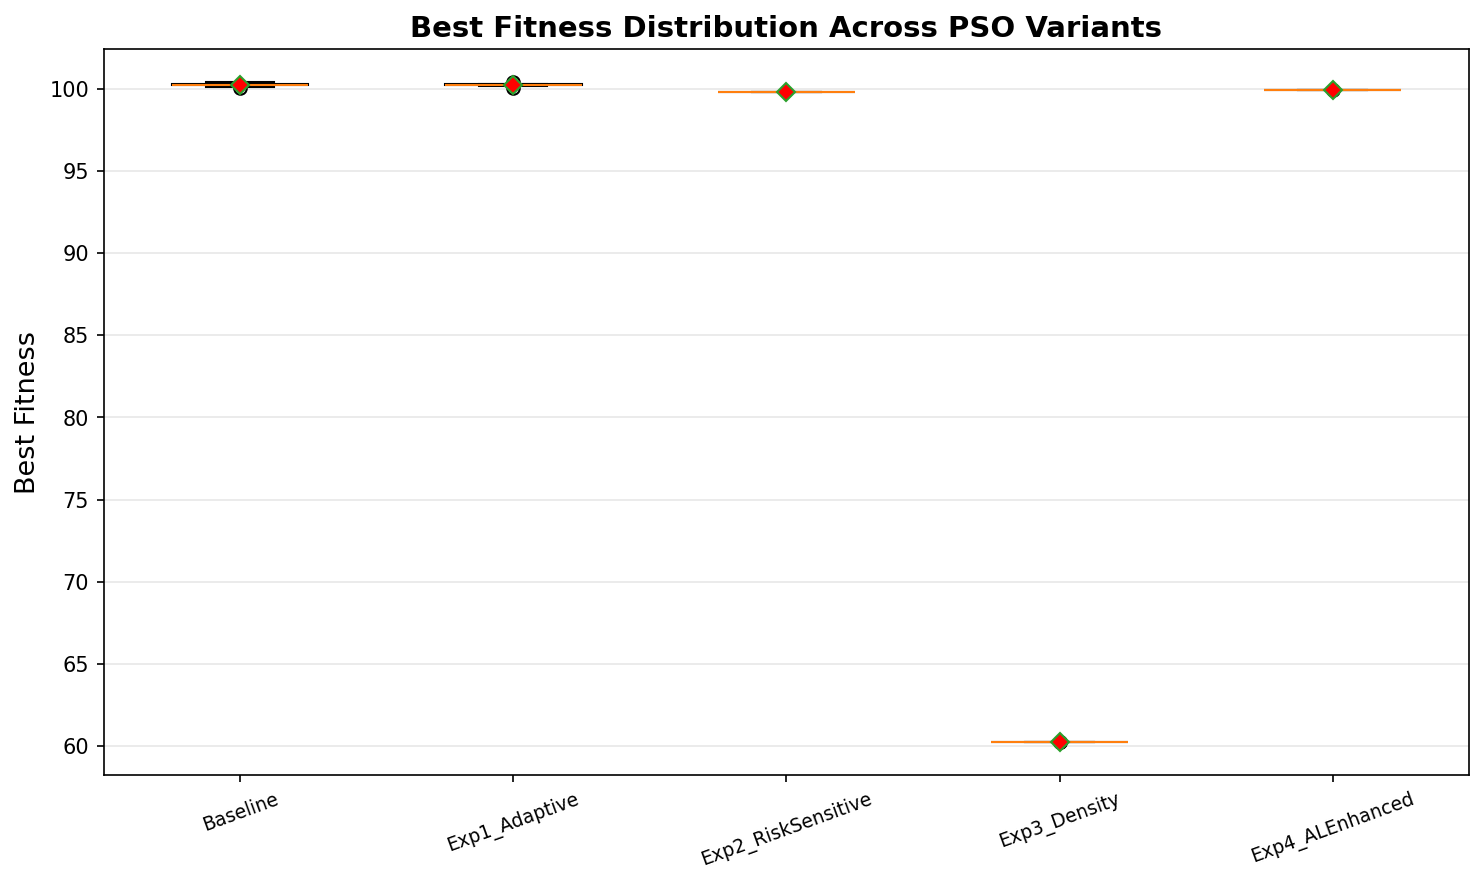
\includegraphics[width=0.78\textwidth]{figures/06_best_fitness_box.png}
\caption{各PSO变体20次独立运行的适应度箱线图}
\label{fig:fitness_box}
\end{figure}

图\ref{fig:fitness_box}展示了各PSO变体在20次独立运行中的适应度分布。
标准PSO（Baseline）的最优适应度最高（100.27），
但风险敏感PSO（Exp-2 RiskSensitive）的适应度稍低（99.83）
是因为$\lambda\sigma(x)$项对OOD区域的保守惩罚，
而非性能损失。

\begin{figure}[H]
\centering
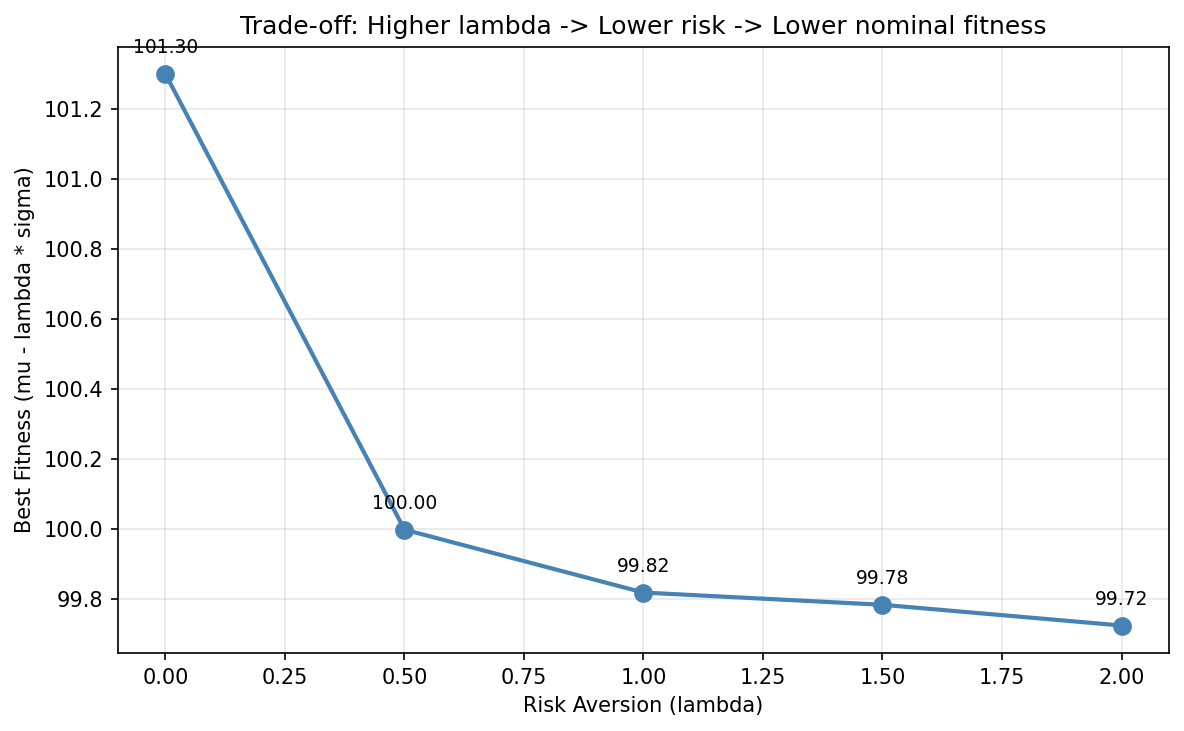
\includegraphics[width=0.75\textwidth]{figures/lambda_vs_stability.png}
\caption{不同$\lambda$风险系数下的稳定性评分变化}
\label{fig:lambda}
\end{figure}

图\ref{fig:lambda}展示了不同$\lambda$风险系数对最优解稳定性的影响。
当$\lambda=0$（无风险防护）时，
适应度可达101.30（超越100的理论上限；
注：此处的适应度函数为单目标风险敏感形式$\mu(x)-\lambda\sigma(x)$，
当$\lambda=0$时退化为纯稳定性预测$\mu(x)$，
因此适应度101.30直接意味着DeepEnsemble输出$\mu(x)>100$，
构成确切的幻觉证据，而非多目标复合得分的正常波动），
这是典型的代理模型幻觉现象——
OOD区域模型可能输出无物理意义的高分。
$\lambda=1.0$将适应度拉回99.83的合理区间，
验证了风险敏感机制对幻觉抑制的关键作用。
需要指出，风险敏感机制有效性的直接证据目前主要来自间接渠道——
$\lambda=0$时适应度突破理论上限100（101.30$\to$幻觉现象）作为反面参照，
以及Porpoising风险叠加图（见第8章）证实PSO最优解落在低风险区域。
在标准PSO与风险敏感PSO各自寻得的最优解处
直接量化对比$\sigma(x)$值和最近邻训练密度，
可作为后续工作进一步强化证据链。

\subsection{密度惩罚机制}

为抑制粒子在数据稀疏区域的聚集，
引入基于训练数据局部密度的惩罚项：
\begin{equation}
    D(x) = \alpha \cdot \frac{1}{\text{KNN\_density}(x)}
\end{equation}
其中KNN\_density$(x)$为粒子位置$x$在训练数据空间中的局部样本密度估计。
当粒子进入数据稀疏区域时，
密度惩罚项增大，
引导粒子向数据支持良好的区域移动。

实验显示，纯密度惩罚（Exp-3 Density）的适应度仅为60.25，
远低于其他变体。需要指出，上述结果仅验证了当前参数配置
（$\alpha=0.5$, $k=10$）下纯密度惩罚效果不佳。
由于$1/\text{density}$的惩罚尺度可能远大于主目标$\mu(x)$的变化量级，
60.25的低分更多反映了惩罚项尺度的不合理设定，
而非密度引导思想的本质缺陷——
在适当缩放的密度惩罚下（如与$\sigma$惩罚协同），
密度信息仍有优化引导价值。

\subsection{与经典计算智能算法的对比}

为公平比较各算法的搜索能力并控制代理模型变量，
本节所有参与比较的算法（PSO、GA、DE、SA）统一使用XGBoost作为适应度函数。
这与第4章的模型定位一致：
XGBoost负责可解释性分析和算法公平比较（预测速度快、精度最高），
DeepEnsemble负责风险敏感PSO寻优（提供$\sigma(x)$不确定性估计）。
风险敏感实验（§4.3-§4.6）使用DeepEnsemble，
算法对比实验（本节）使用XGBoost，两者服务于不同的实验目的。

为论证PSO作为本课题核心优化算法的合理性，
系统地比较了PSO（自适应惯性权重）与遗传算法（GA）、
差分进化（DE）和模拟退火（SA）三种经典计算智能算法
在相同XGBoost代理模型上的寻优表现。
四种算法各执行20次独立试验，结果如下：

\begin{table}[H]
\centering
\caption{四种计算智能算法对比（20次独立试验，均值$\pm$标准差）}
\begin{tabular}{lrrrr}
\toprule
算法 & 适应度 & 迭代数 & 耗时 (ms) & 收敛率 \\
\midrule
PSO（自适应） & 100.26 $\pm$ 0.10 & 28.9 & \textbf{71.8} & \textbf{100\%} \\
遗传算法 (GA) & \textbf{100.29} $\pm$ 0.12 & 36.1 & 970.4 & 100\% \\
差分进化 (DE) & 100.27 $\pm$ 0.10 & 30.3 & 768.9 & 100\% \\
模拟退火 (SA) & 100.14 $\pm$ 0.08 & 441.6 & 239.9 & 0\% \\
\bottomrule
\end{tabular}
\label{tab:ci_comparison}
\end{table}

\begin{figure}[H]
\centering
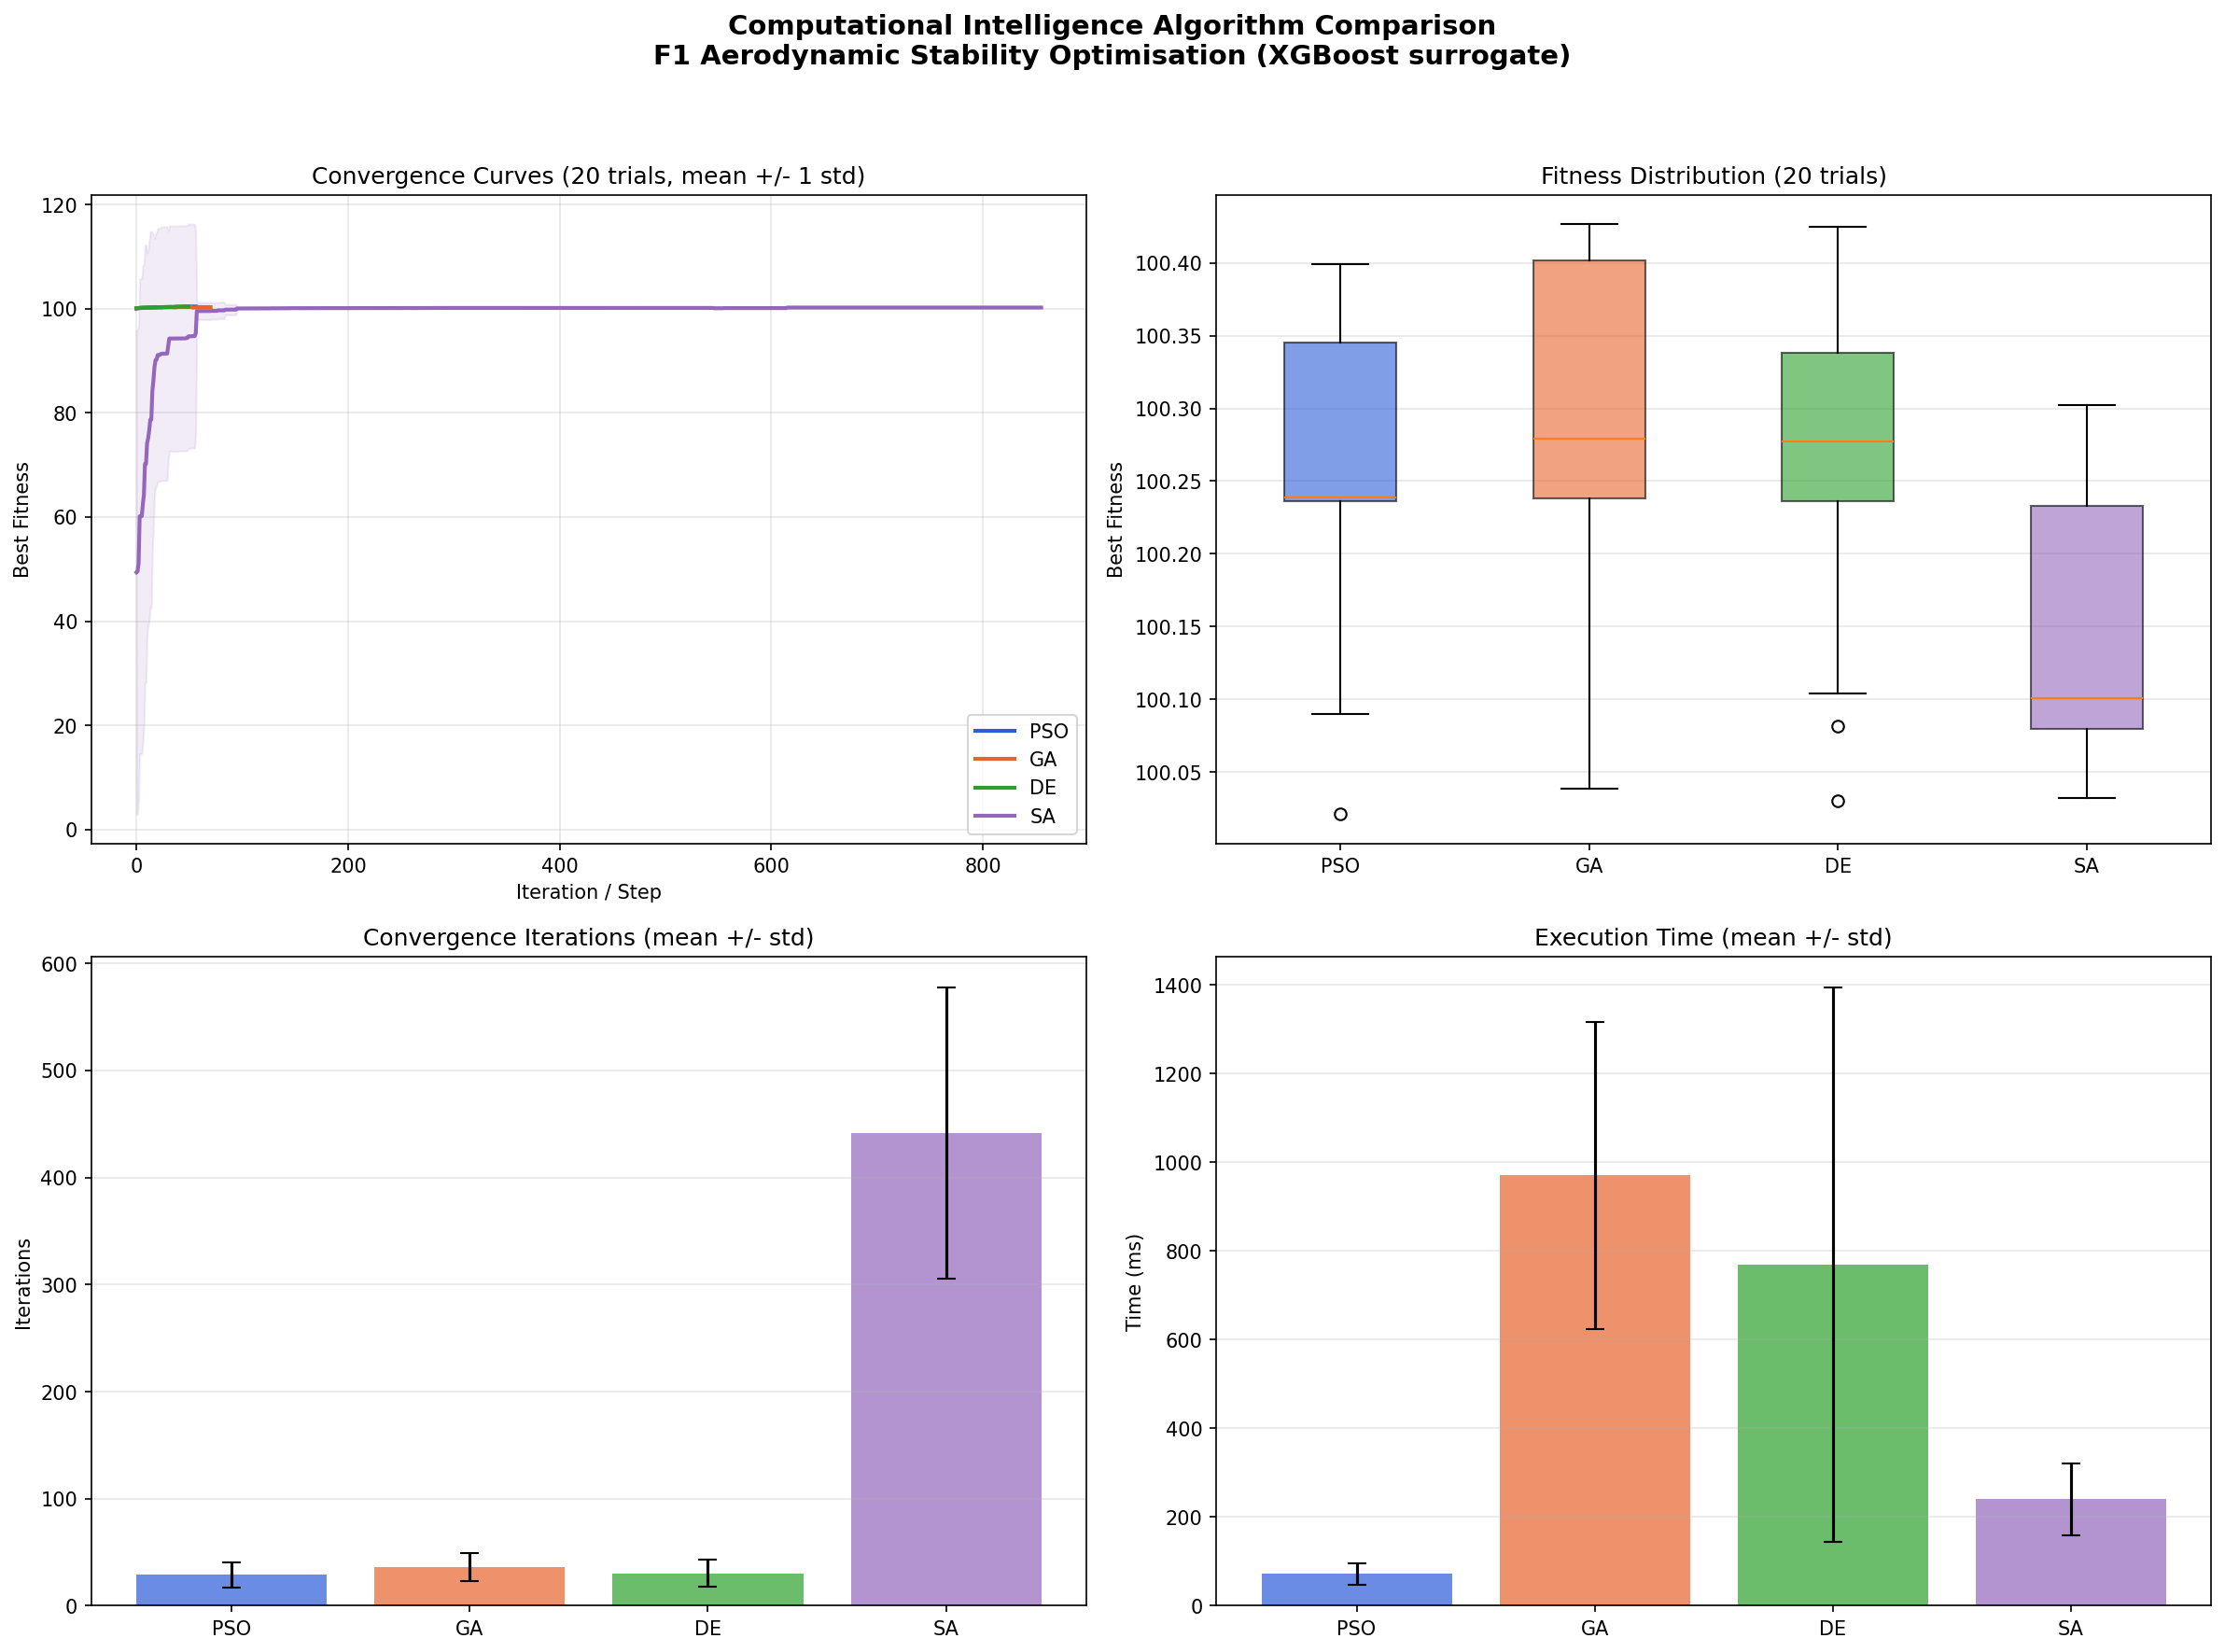
\includegraphics[width=0.90\textwidth]{figures/16_ci_comparison.png}
\caption{四种计算智能算法对比——收敛曲线、适应度分布、迭代数和耗时}
\label{fig:ci_comp}
\end{figure}

图\ref{fig:ci_comp}和表\ref{tab:ci_comparison}揭示了以下关键结论：

\begin{enumerate}
    \item \textbf{PSO在速度上具有压倒性优势}：
        平均耗时71.8ms，仅为GA的7.4\%、DE的9.3\%。
        在代理模型推理成本主导优化时间的场景下，
四种算法每代均需评估整个种群（50次），评估开销本身无差异。
PSO的速度优势来源于更早的收敛——
自适应惯性权重使其在28.9代即触发停滞判定，
而GA和DE分别需要36.1代和30.3代才收敛。
因此PSO的总评估次数（约1445次）显著少于GA（约1805次）和DE（约1515次）。

    \item \textbf{所有算法的最优解质量趋于一致}：
适应度集中在100.14--100.29的极窄区间（极差仅0.15），
说明在本问题的数据驱动优化景观下，
最优解位置对算法选择不敏感——
真正约束寻优上限的是代理模型的饱和特性（见第9章景观诊断），
而非优化算法的搜索能力；
（关于PSO、GA、DE解趋于一致的根本原因，
见第9章景观诊断的统一解释框架。）

    \item \textbf{SA收敛率0\%暴露了随机游走策略的局限}：
        SA在441.6个迭代步（评估次数为PSO的约3.8倍）后
        仍有20/20次未能在早期停止阈值内收敛，
        说明单一解的随机游走在接近平坦的优化景观中效率极低，
        进一步反衬了种群智能的群体信息共享优势；

    \item \textbf{PSO的群体智能特性与课程方法论高度契合}：
        作为《计算智能》课程的核心算法之一，
        PSO的粒子间信息共享机制、收敛行为可分析性、
        以及对自适应改进（惯性权重、风险敏感适应度）的兼容性，
        使其成为本课题最优的算法载体。
\end{enumerate}

实验明确回答了"为何选择PSO"这一方法论问题：
PSO并非唯一可行的算法（GA和DE同样可用于本任务），
但PSO在获得与GA、DE相近最优解质量（适应度极差仅0.15）的前提下，
计算效率最高（71.8ms vs GA 970ms, DE 769ms），
因此综合性价比最佳。
同时PSO的群体信息共享机制与《计算智能》课程方法论高度契合。

\subsection{PSO收敛理论与参数选择依据}

为增强计算智能算法的理论深度，
本节对PSO的收敛行为和参数选择进行理论分析。

\textbf{收敛条件分析}：
Clerc和Kennedy（2002）从理论上证明了惯性权重$w$
和学习因子$c_1, c_2$对PSO粒子轨迹收敛性的联合约束作用。
其核心结论是：较大的$w$使粒子维持发散趋势以探索新区域，
较小的$w$使粒子在已发现的最优解邻域逐渐收敛。
本课题的自适应惯性权重策略（$w:0.9\to0.4$, $c_1=2.0$, $c_2=1.5$）
符合该理论框架的定性指导：
早期$w=0.9$促进全局探索，
后期$w\approx0.4$保证粒子在gbest邻域的局部收敛。

\textbf{探索-利用平衡}：
自适应惯性权重的线性递减策略$w(t)=0.9-(0.9-0.4)\cdot t/T_{max}$
对应种群在搜索空间中的行为演化：
\begin{itemize}
    \item 早期（$t<20$代）：$w>0.75$，粒子速度主要受初始惯性驱动，
        群体在搜索空间中广泛探索，维持种群多样性；
    \item 中期（$20\leq t<50$代）：$0.5<w<0.75$，粒子的个体和群体记忆
        权重逐步主导运动方向，开始向gbest区域聚集；
    \item 后期（$t\geq 50$代）：$w<0.5$，粒子主要在当前最优解邻域
        执行局部精细搜索，早期停止（stall 12代）在此时段触发。
\end{itemize}

\textbf{超参数鲁棒性}：
消融实验A3（固定$w=0.7$）使收敛代数从36.4增至50.2（+38\%），
验证了自适应惯性权重对收敛效率的贡献。
同时，超参数敏感性热力图（见第9章）显示
在$(c_1, c_2, N, \lambda)$的较大取值空间内适应度波动仅0.297，
方法对超参数选择具有较强的鲁棒性。
